\documentclass[9pt]{beamer}
\usepackage{fontspec}
\usepackage[english,bulgarian]{babel}
\usepackage{xcolor}
\usepackage{amsmath}
\usepackage{mathtools} 
\usepackage{nccmath}
\usepackage{caption}
\usepackage{subfig}
\usepackage{animate}
\usepackage{xmpmulti}

\defaultfontfeatures{Ligatures=TeX}
\newfontfamily\cyrillicfont{Comfortaa-Regular}
\newfontfamily\cyrillicfonttt{Comfortaa-Regular}
\newfontfamily\fontcomic[NFSSFamily=roboto]{Roboto}
\setsansfont{Comfortaa-Regular}

\graphicspath{ {./resources/} }

\newcommand{\Q}[1]{\left[#1\right]}
\newcommand{\B}[1]{\left(#1\right)}


\usetheme{metropolis}
% \usetheme{boxes}

\begin{document}
\section{Разпознаване на емоции в сигнали от реч и ЕЕГ}
\begin{frame}{Нулева зона}
    \pause
    \begin{center}
        Първични и вторични канали за изразяване на емоция
    \end{center}
    \pause 
    \begin{itemize}
        \item[$\ $] Първичен канал - ЕЕГ
        \pause
        \item[$\ $] Вторичен канал - реч
        \begin{itemize}
            \pause 
            \item Експлицитно и имплицитно общуване
            \pause
            \item Прозодия
        \end{itemize}
        \pause
        \item Съчетаване на първичен (ЕЕГ) и вторичен (реч) канал
    \end{itemize}
\end{frame}

\section{Емоции}
\setbeamercolor{background canvas}{bg=white}
\begin{frame}
    \begin{center}
        \only<1>{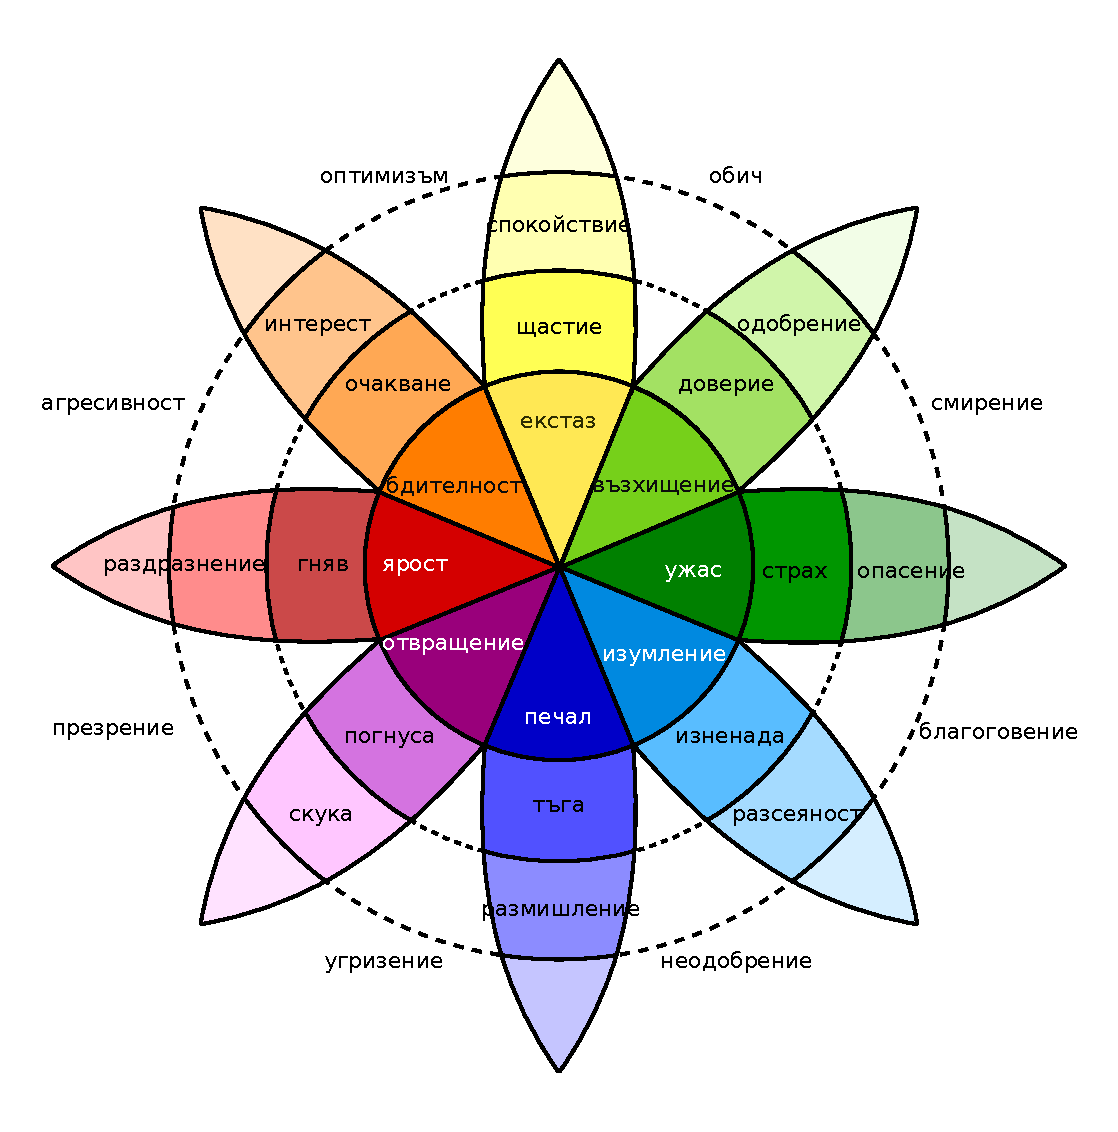
\includegraphics[width=0.8\textwidth]{plutchik}}%
        \only<2>{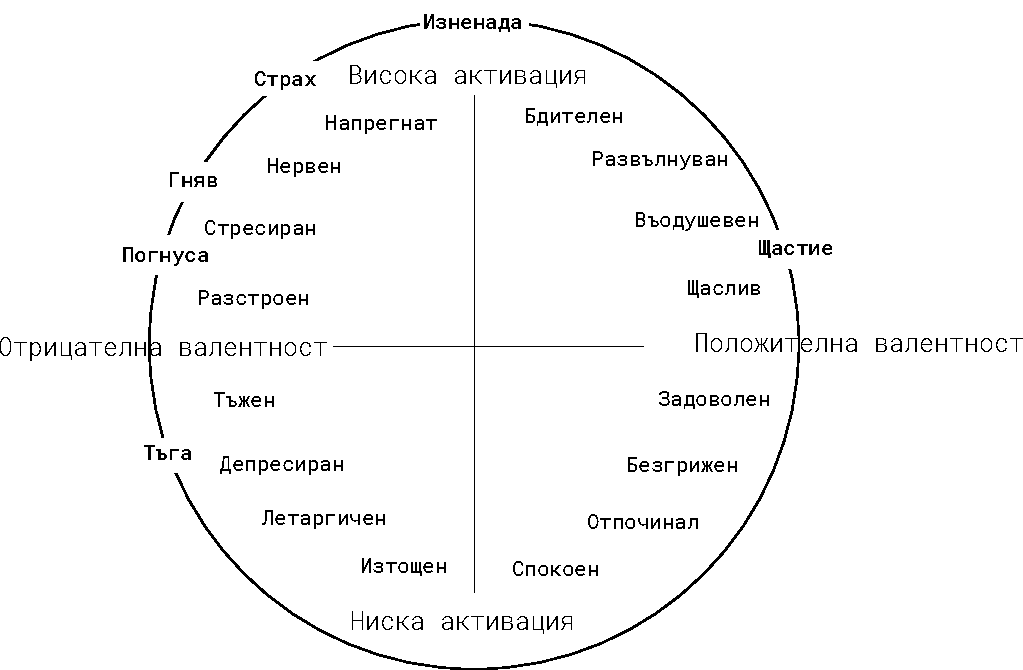
\includegraphics[width=\textwidth]{valence_arousal}}
    \end{center}
\end{frame}

\setbeamercolor{background canvas}{bg=white}
\begin{frame}
        \only<1>{
            \begin{columns}[T] % align columns
            \begin{column}{.38\textwidth}
            \end{column}%
            \hfill%
            \begin{column}{.60\textwidth}
                \vspace{1cm}
                \begin{center}
                    
\includegraphics[width=\textwidth]{valence_arousal_empty}%
                \end{center}
            \end{column}%
        \end{columns}
        }

        \only<2>{
            \begin{columns}[T] % align columns
            \begin{column}{.38\textwidth}
                \begin{itemize}
                    \item Гняв
                \end{itemize}
            \end{column}%
            \hfill%
            \begin{column}{.60\textwidth}
                \vspace{1cm}
                \begin{center}
                    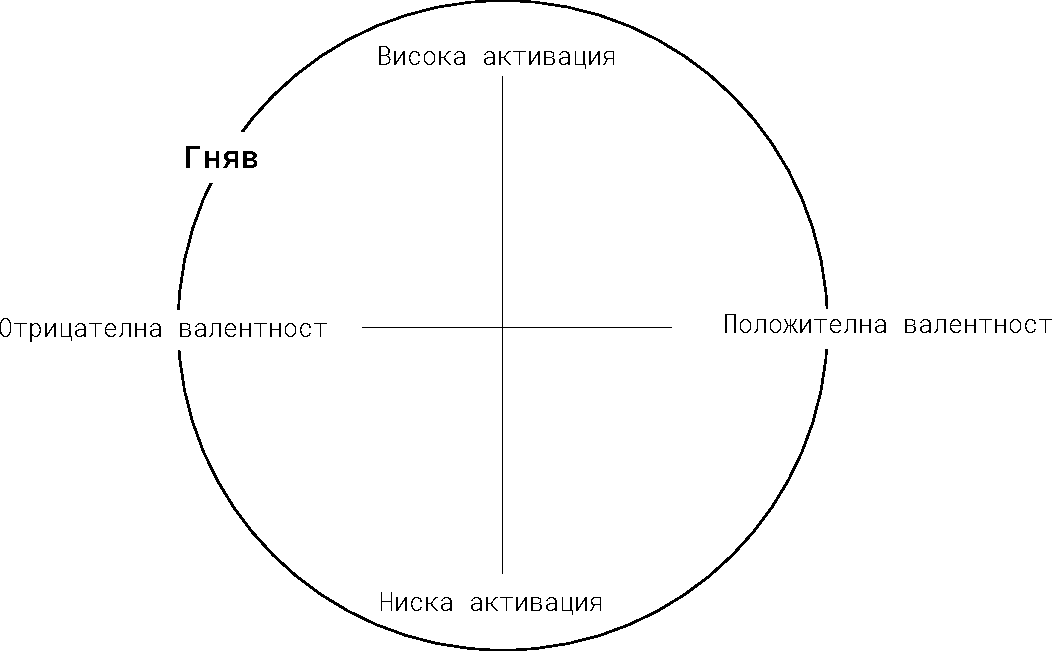
\includegraphics[width=\textwidth]{valence_arousal_a}%
                \end{center}
            \end{column}%
        \end{columns}
        }

        \only<3>{
            \begin{columns}[T] % align columns
            \begin{column}{.38\textwidth}
                \begin{itemize}
                    \item Гняв
                    \item Щастие
                \end{itemize}
            \end{column}%
            \hfill%
            \begin{column}{.60\textwidth}
                \vspace{1cm}
                \begin{center}
                    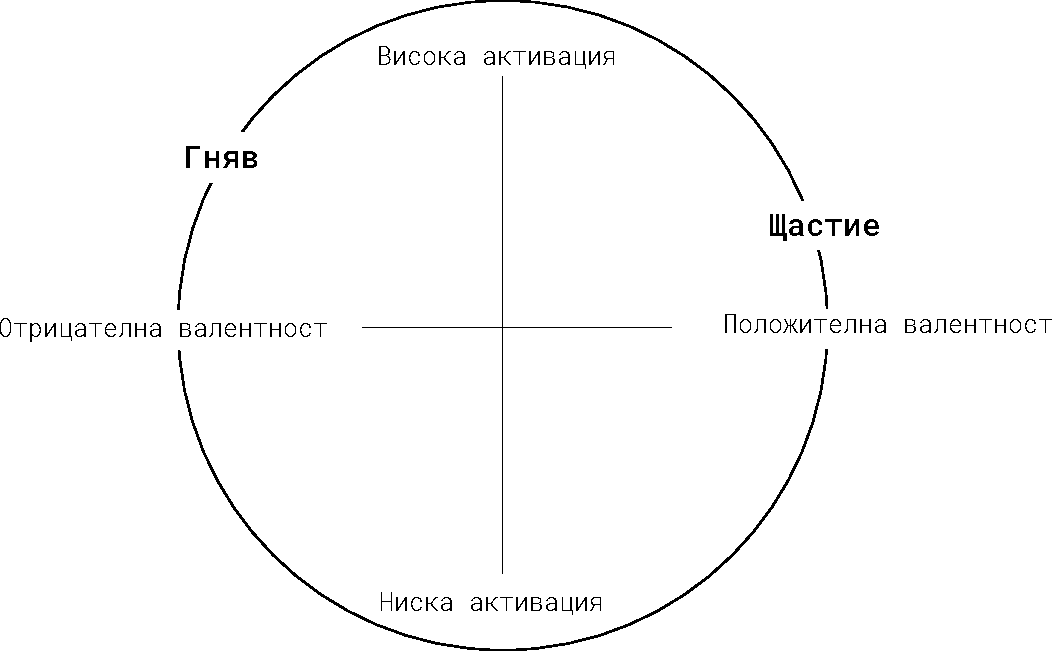
\includegraphics[width=\textwidth]{valence_arousal_ah}%
                \end{center}
            \end{column}%
        \end{columns}
        }

        \only<4>{
            \begin{columns}[T] % align columns
            \begin{column}{.38\textwidth}
                \begin{itemize}
                    \item Гняв
                    \item Щастие
                    \item Неутрална емоция
                \end{itemize}
            \end{column}%
            \hfill%
            \begin{column}{.60\textwidth}
                \vspace{1cm}
                \begin{center}
                    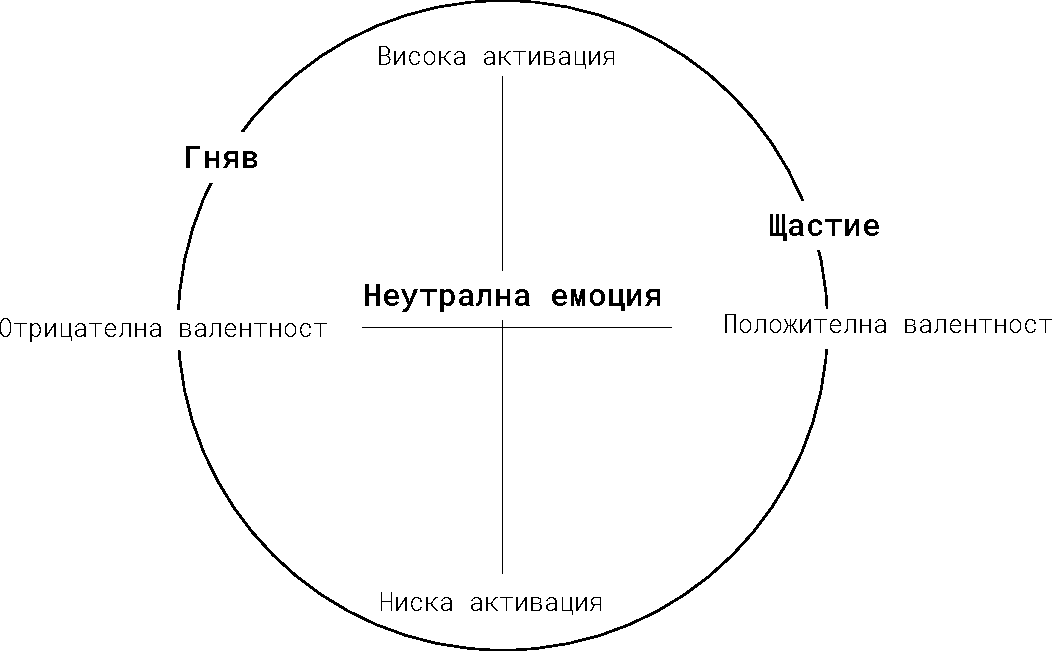
\includegraphics[width=\textwidth]{valence_arousal_ahn}%
                \end{center}
            \end{column}%
        \end{columns}
        }

        \only<5>{
            \begin{columns}[T] % align columns
            \begin{column}{.38\textwidth}
                \begin{itemize}
                    \item Гняв
                    \item Щастие
                    \item Неутрална емоция
                    \item Тъга
                \end{itemize}
            \end{column}%
            \hfill%
            \begin{column}{.60\textwidth}
                \vspace{1cm}
                \begin{center}
                    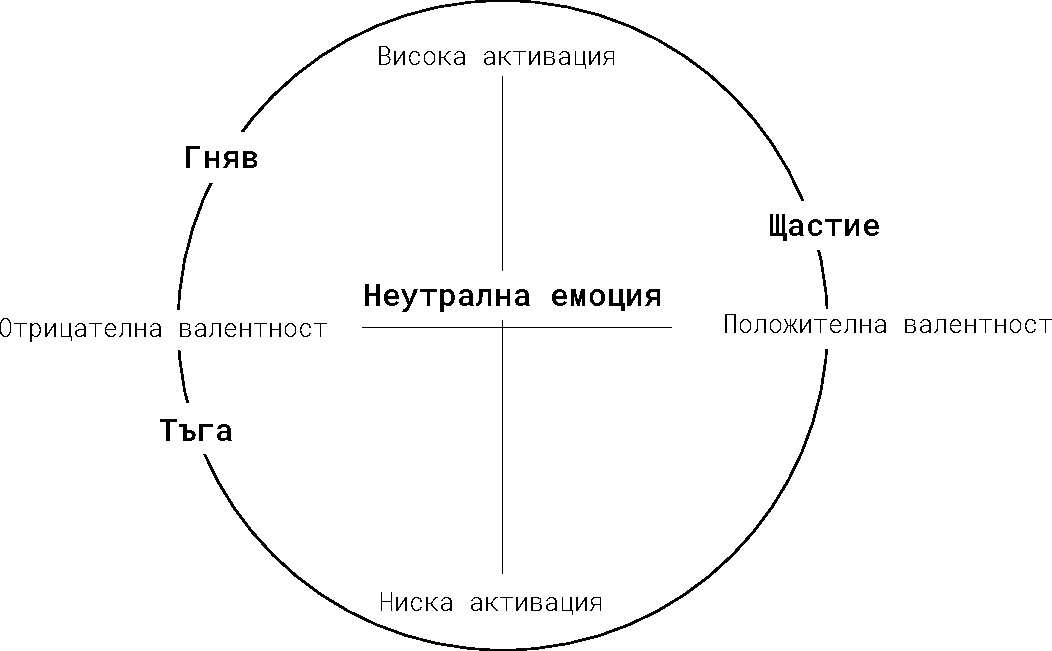
\includegraphics[width=\textwidth]{valence_arousal_ahns}%
                \end{center}
            \end{column}%
        \end{columns}
        }
\end{frame}

\section{Реч}
\begin{frame}[b]
    \only<1>{
        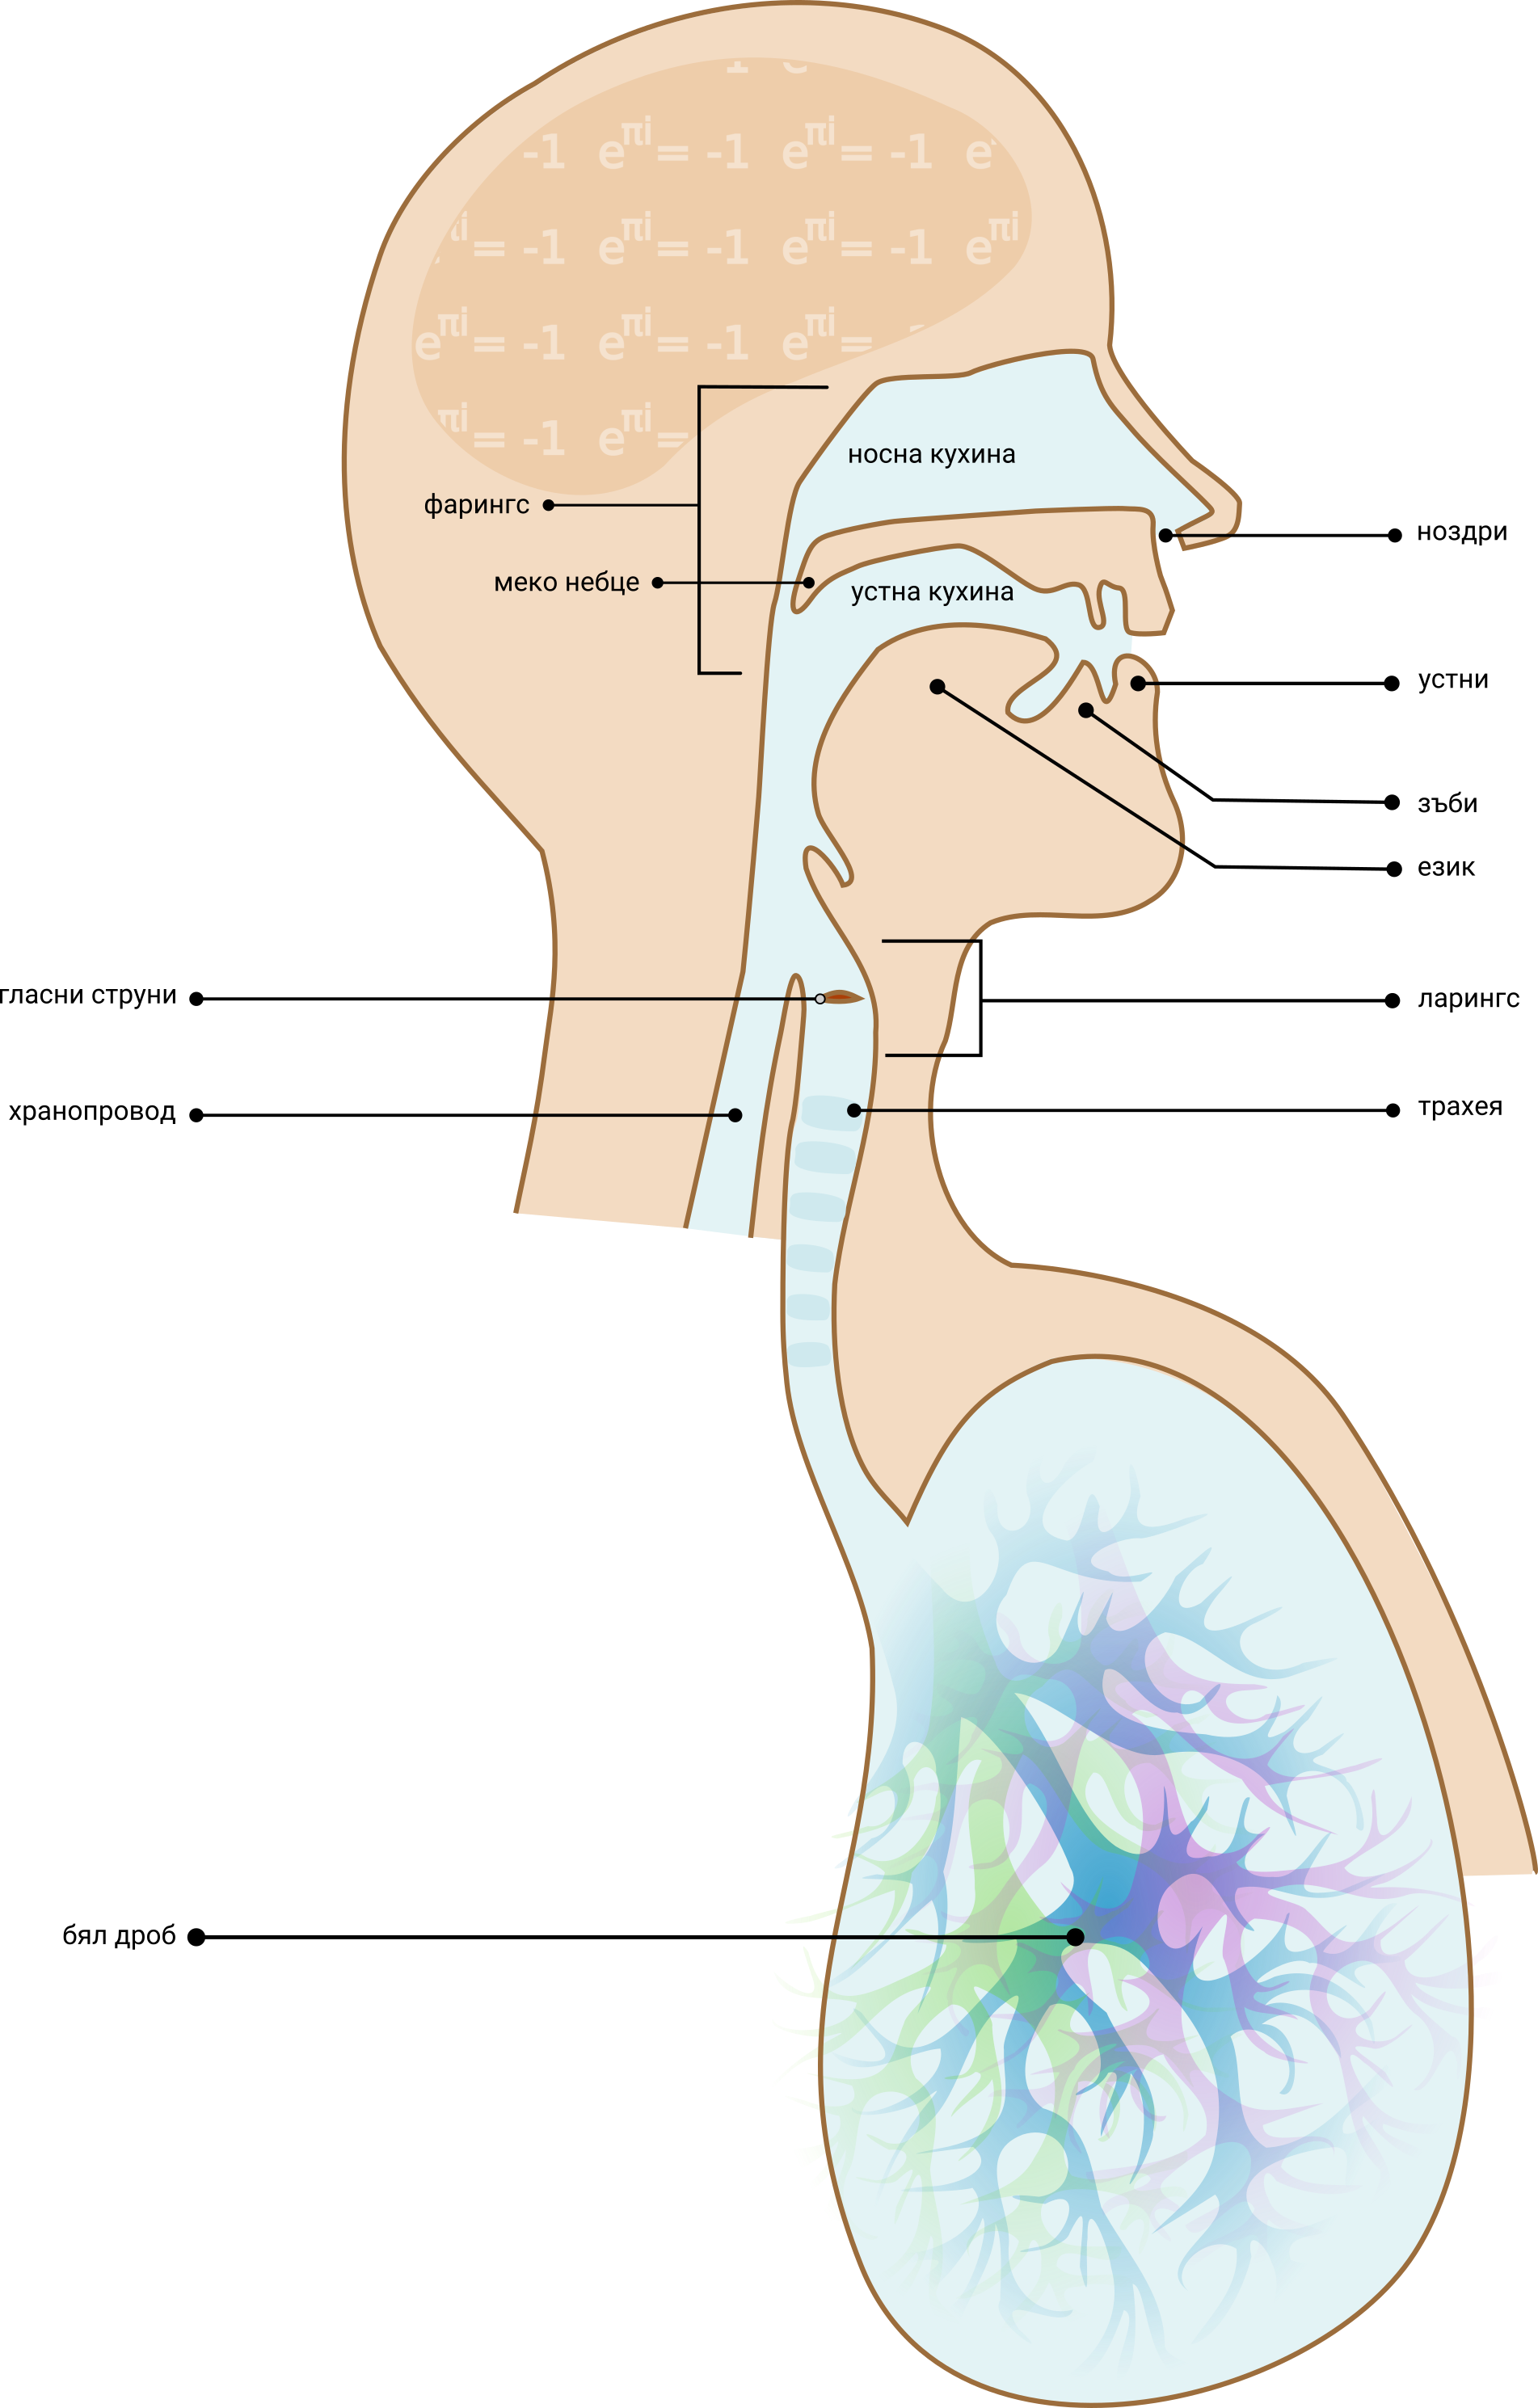
\includegraphics[width=0.48\paperwidth]{physics}%
        \hfill
        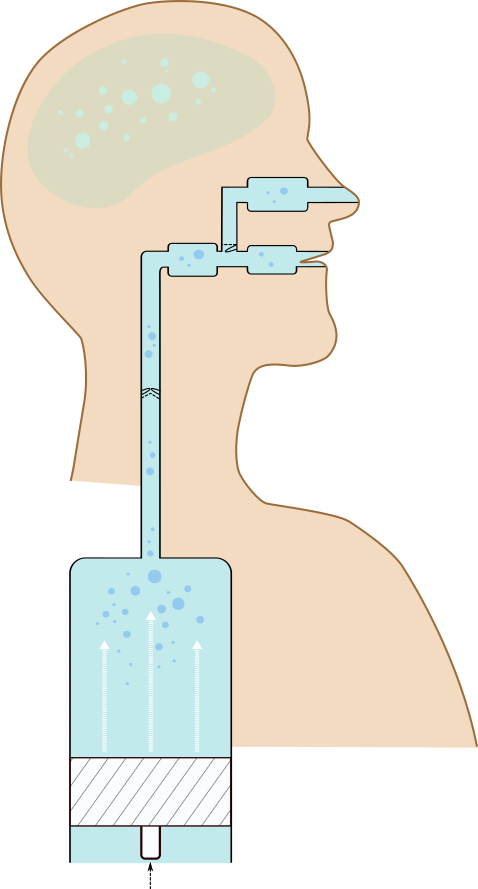
\includegraphics[width=0.28\paperwidth]{tubes}
    }
    \only<2>{
        \centering{
            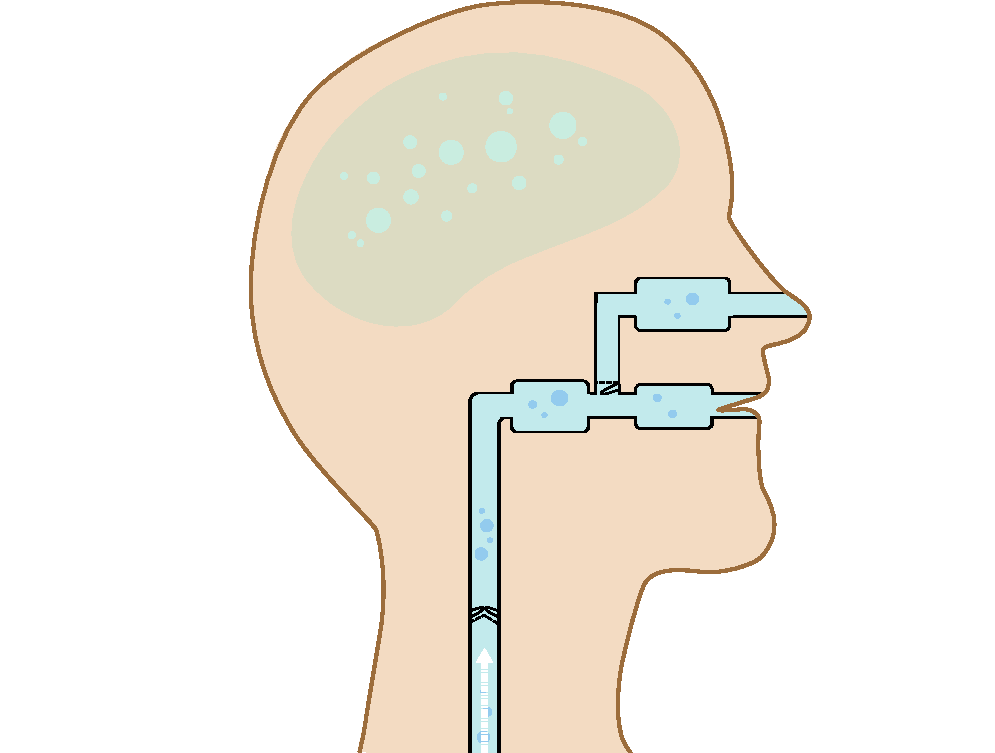
\includegraphics[height=\textheight]{glottis}%
        }
    }
\end{frame}

\begin{frame}
    \begin{itemize}
        \only<1>{
                 \item  Глотисът \alert{g} трепти, вокалният тракт \alert{v} филтрира сигнала, и вълната излиза и допълнително се променя от устните \alert{r}
                 }
        \only<2->{
                    \item  Глотисът $\textbf{g}$ трепти, вокалният тракт $\textbf{v}$ филтрира сигнала, и вълната излиза и допълнително се променя от устните $\textbf{r}$
                 }
        \only<2>{
                 \item[$\ $] Ако  $g(t) \xleftrightarrow{\mathcal{F}\mathcal{S}} \mathcal{G}(z), v(t) \xleftrightarrow{\mathcal{F}\mathcal{S}} \mathcal{V}(z), r(t) \xleftrightarrow{\mathcal{F}\mathcal{S}} \mathcal{R}(z)$, а сигналът, който получаваме накрая, $y(t)=g(t)\ast v(t) \ast r(t), y(t) \xleftrightarrow{\mathcal{F}\mathcal{S}} \mathcal{Y}(z)$, е изпълнено, че
                 }
        \only<3->{
                    \item[$\ $] Ако  $g(t) \xleftrightarrow{\mathcal{F}\mathcal{S}} \mathcal{G}(z), v(t) \xleftrightarrow{\mathcal{F}\mathcal{S}} \mathcal{V}(z), r(t) \xleftrightarrow{\mathcal{F}\mathcal{S}} \mathcal{R}(z)$, а сигналът, който получаваме накрая, $y(t)=g(t)\ast v(t) \ast r(t), y(t) \xleftrightarrow{\mathcal{F}\mathcal{S}} \mathcal{Y}(z)$, е изпълнено, че
                 }
        \only<3>{
                 \item $\mathcal{Y}(z) = \mathcal{G}(z) \mathcal{V}(z) \mathcal{R}(z)$
                }
        \only<4>{
            \item $\mathcal{Y}(z) = \mathcal{G}(z) \alert{\mathcal{V}(z) \mathcal{R}(z)}$
        }  
        \only<5>{
                \item $\mathcal{Y}(z) = \mathcal{G}(z) \mathcal{H}(z)$
        }
    \end{itemize}
\end{frame}

\begin{frame}[t]
    \begin{itemize}
        \only<1> {
            \item[$\ $] $\alert{\mathcal{Y}(z) = \mathcal{G}(z) \mathcal{H}(z)}$
        }
        \only<2-> {
            \item[$\ $] $\mathcal{Y}(z) = \mathcal{G}(z) \mathcal{H}(z)$
        }
        \only<2> {
            \item Модел на тръбите
        }
        \only<3-> {
            \item Модел на тръбите
        }
        \only<3>{\item Уравнения на Навие-Стокс:

            \begin{flalign*}
                -\frac{\partial\rho}{\partial x} & = \frac{\rho}{A} \frac{\partial u}{\partial t} && \\
                -\frac{\partial u}{\partial x} & = \frac{A}{\rho c^2} \frac{\partial \rho}{\partial t} && 
            \end{flalign*}
        }
        \only<4->{\item Уравнения на Навие-Стокс:
        
            \begin{flalign*}
                -\frac{\partial\rho}{\partial x} & = \frac{\rho}{A} \frac{\partial u}{\partial t} && \\
                -\frac{\partial u}{\partial x} & = \frac{A}{\rho c^2} \frac{\partial \rho}{\partial t} && 
            \end{flalign*}
        }
        \only<4>{\item $\mathcal{Y}(z) = \mathcal{G}(z) \cfrac{\sum\limits_{m=0}^{M} b_m z^{-m} }{\sum\limits_{k=0}^{K} a_k z^{-k}}$}

    \end{itemize}
\end{frame}

\begin{frame}[t]
    \begin{itemize}
        \only<1> {
            \item[$\ $] $\mathcal{Y}(z) = \mathcal{G}(z) \mathcal{H}(z)$
        }
        \only<2-> {
            \item[$\ $] $\mathcal{Y}(z) = \mathcal{G}(z) \mathcal{H}(z)$
        }
        \only<2> { \item $log(|\mathcal{Y}(z)|) = log(|\mathcal{G}(z)|) + log(|\mathcal{H}(z)|)$
        }
        \only<3-> {
            \item $log(|\mathcal{Y}(z)|) = log(|\mathcal{G}(z)|) + log(|\mathcal{H}(z)|)$
        }
        \only<3> {
            \begin{columns}
                \begin{column}{0.48\textwidth}
                     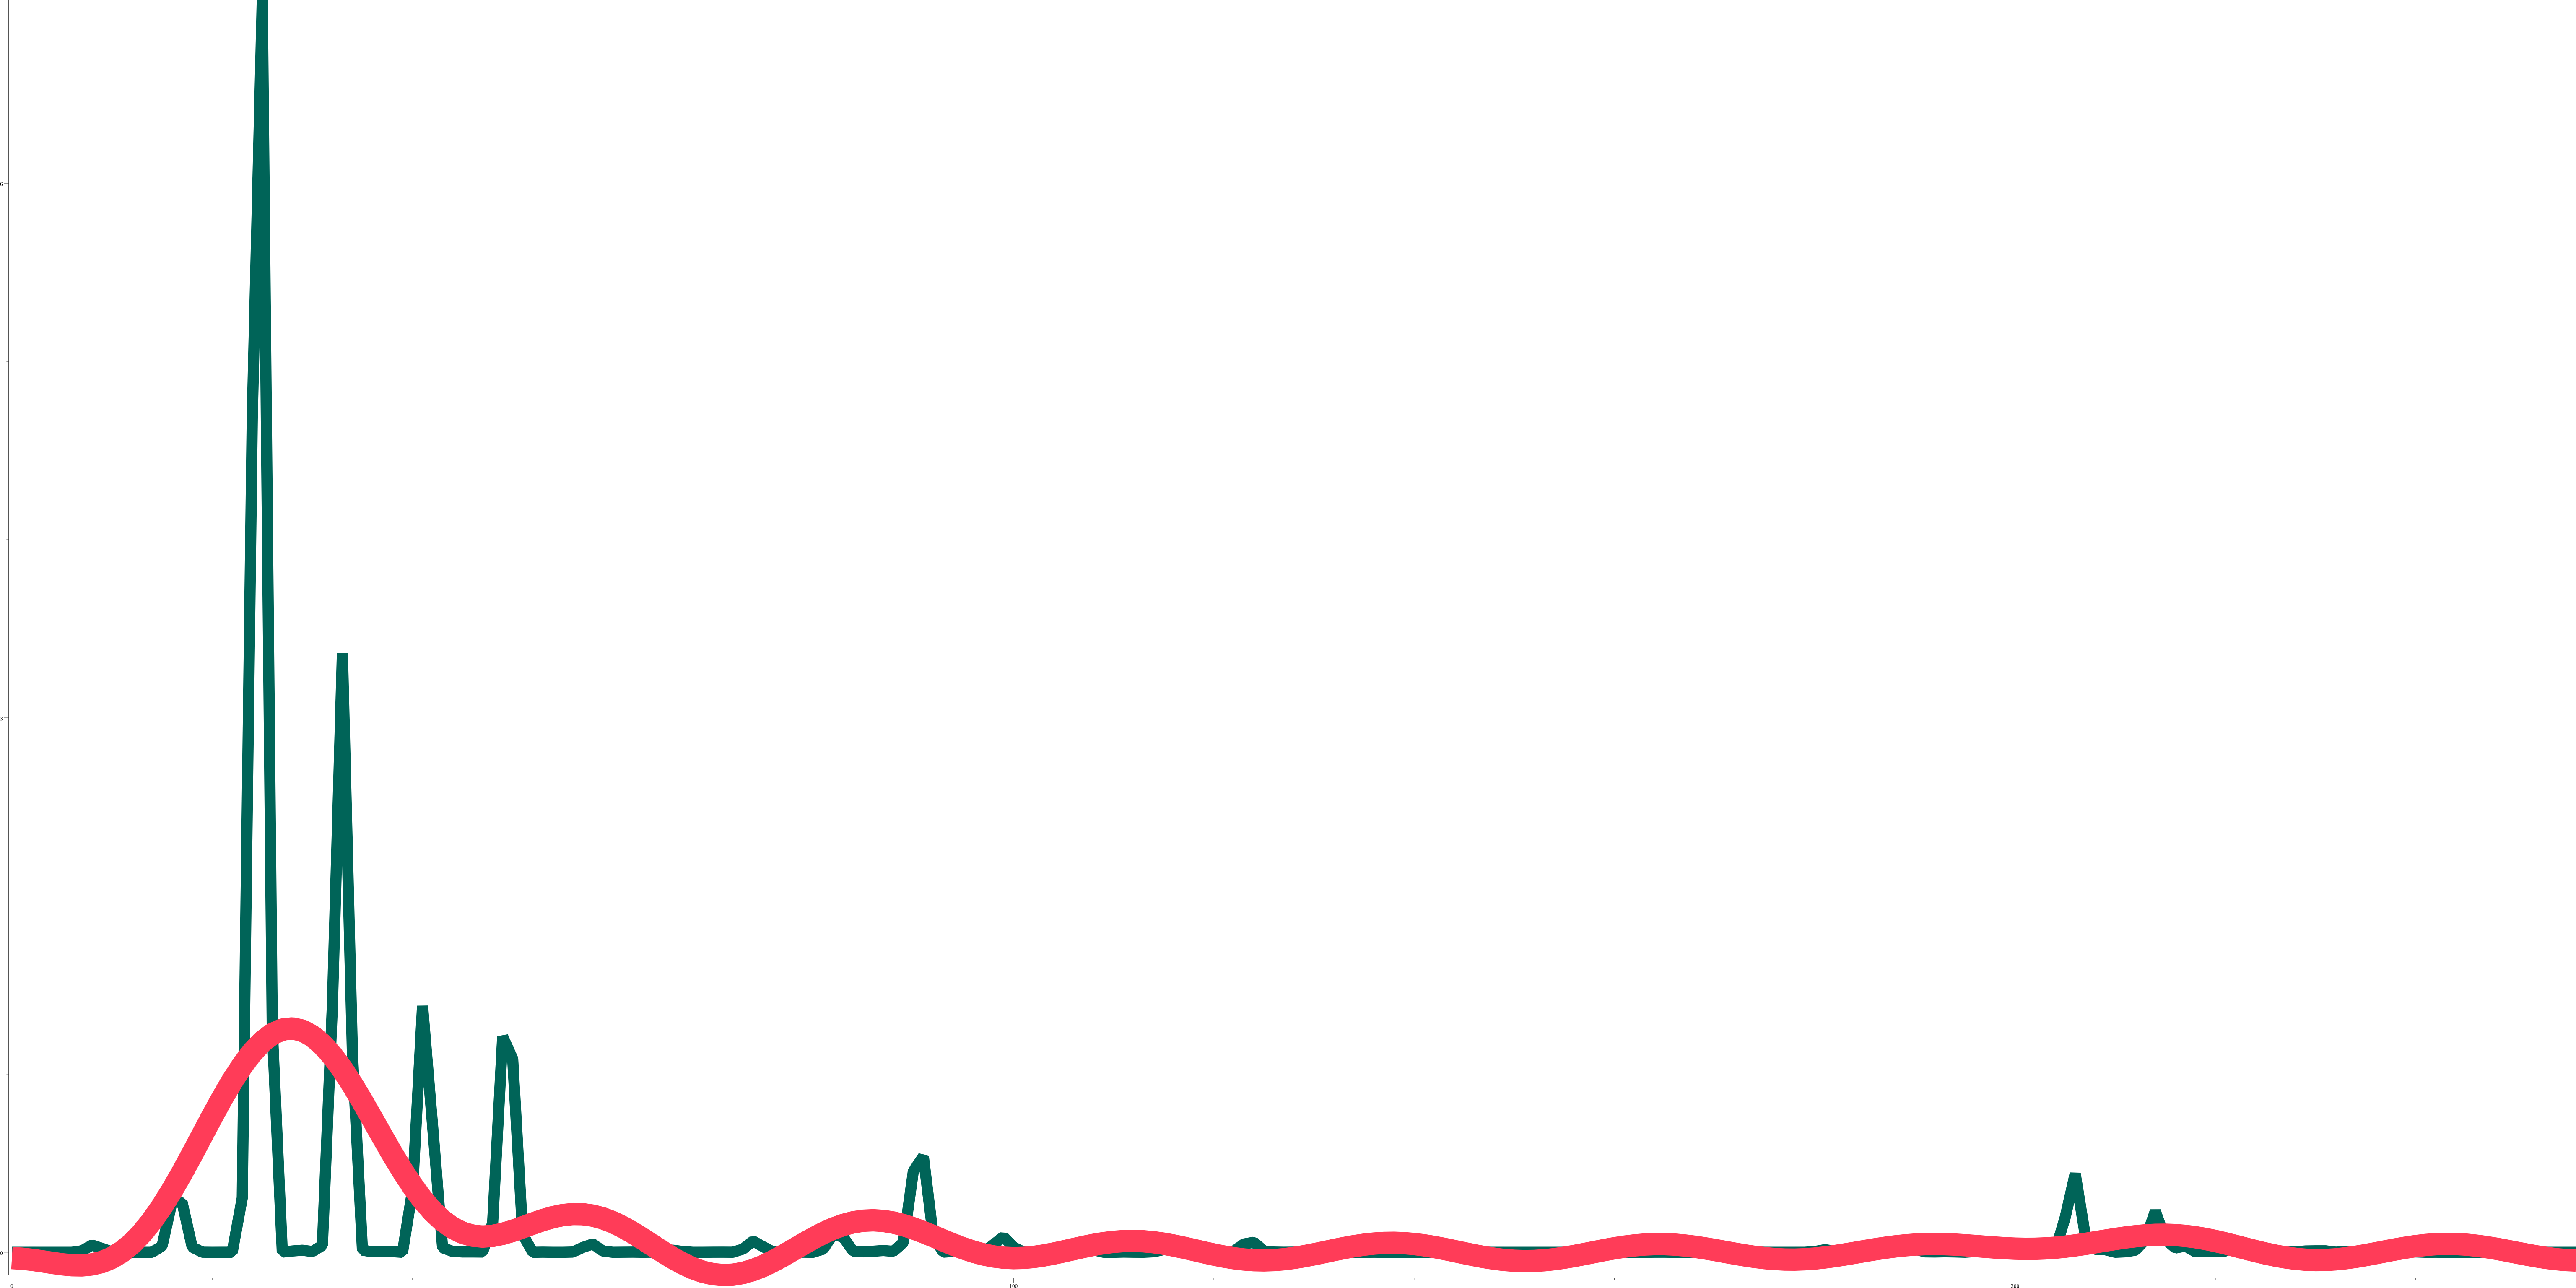
\includegraphics[width=\textwidth]{aaaa.png}
                \end{column}
                \pause
                \hfill
                \begin{column}{0.48\textwidth}
                    %  \includegraphics[width=\textwidth]{aaaa_log.png}
                \end{column}
            \end{columns}
        }
        \only<4> {
                \begin{columns}
                    \begin{column}{0.48\textwidth}
                         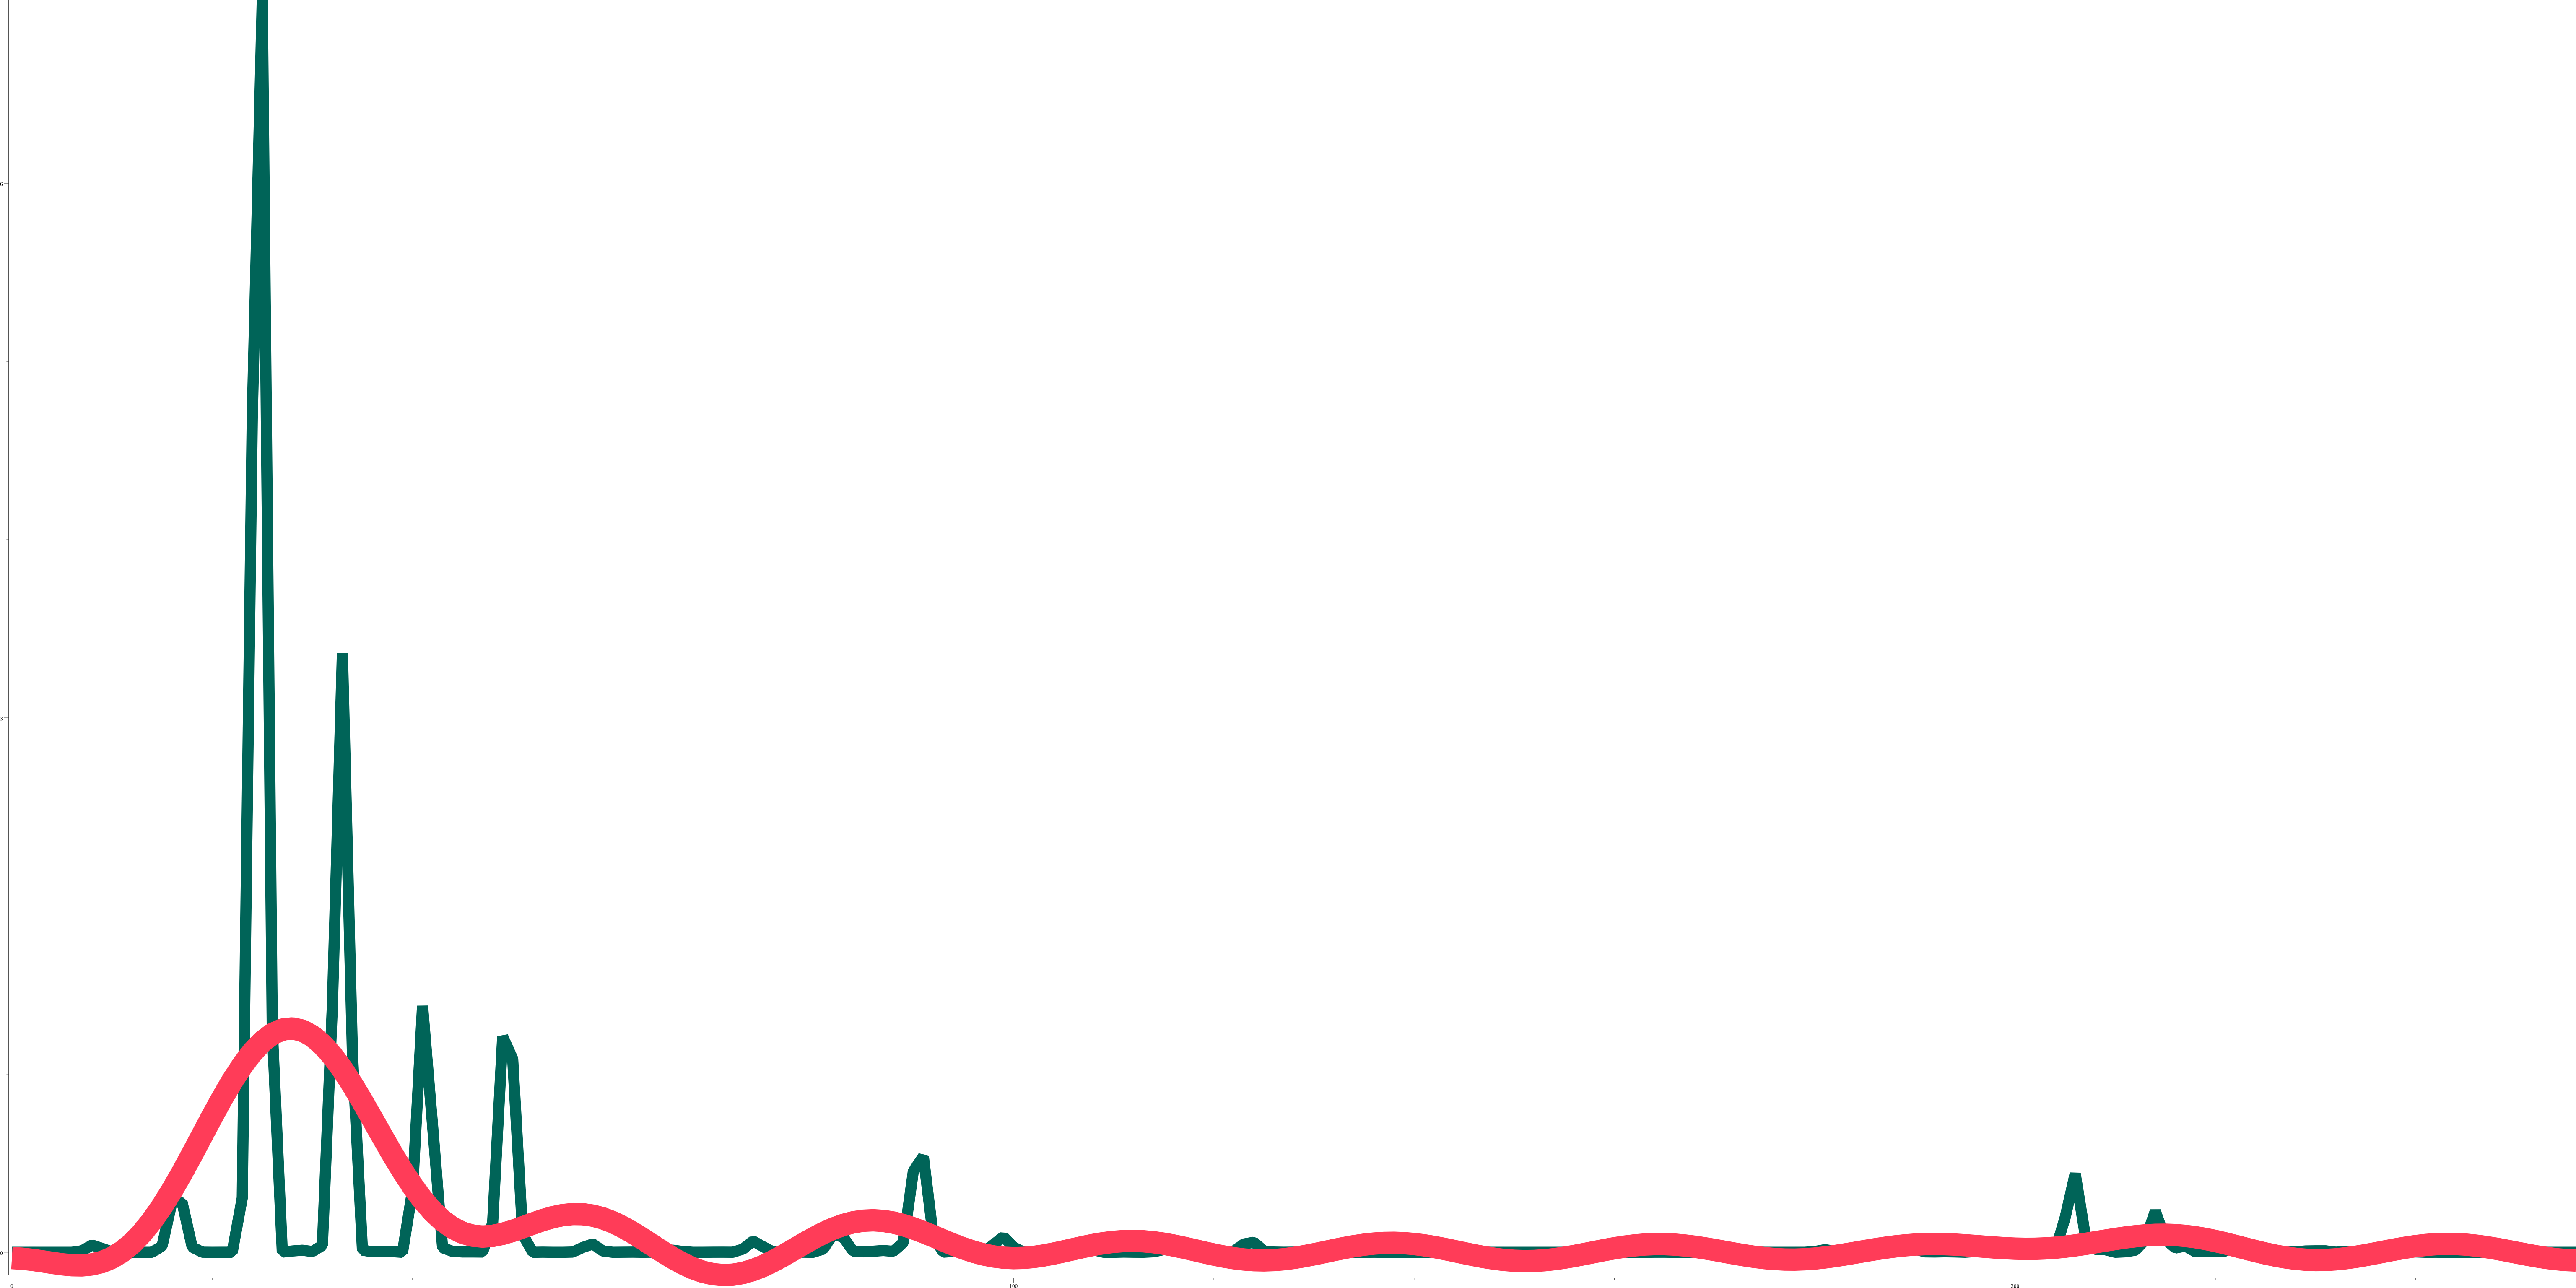
\includegraphics[width=\textwidth]{aaaa.png}
                    \end{column}
                    \pause
                    \hfill
                    \begin{column}{0.48\textwidth}
                         \includegraphics[width=\textwidth]{aaaa_log.png}
                    \end{column}
                \end{columns}
        }
        \only<5-> {
                \begin{columns}
                    \begin{column}{0.48\textwidth}
                         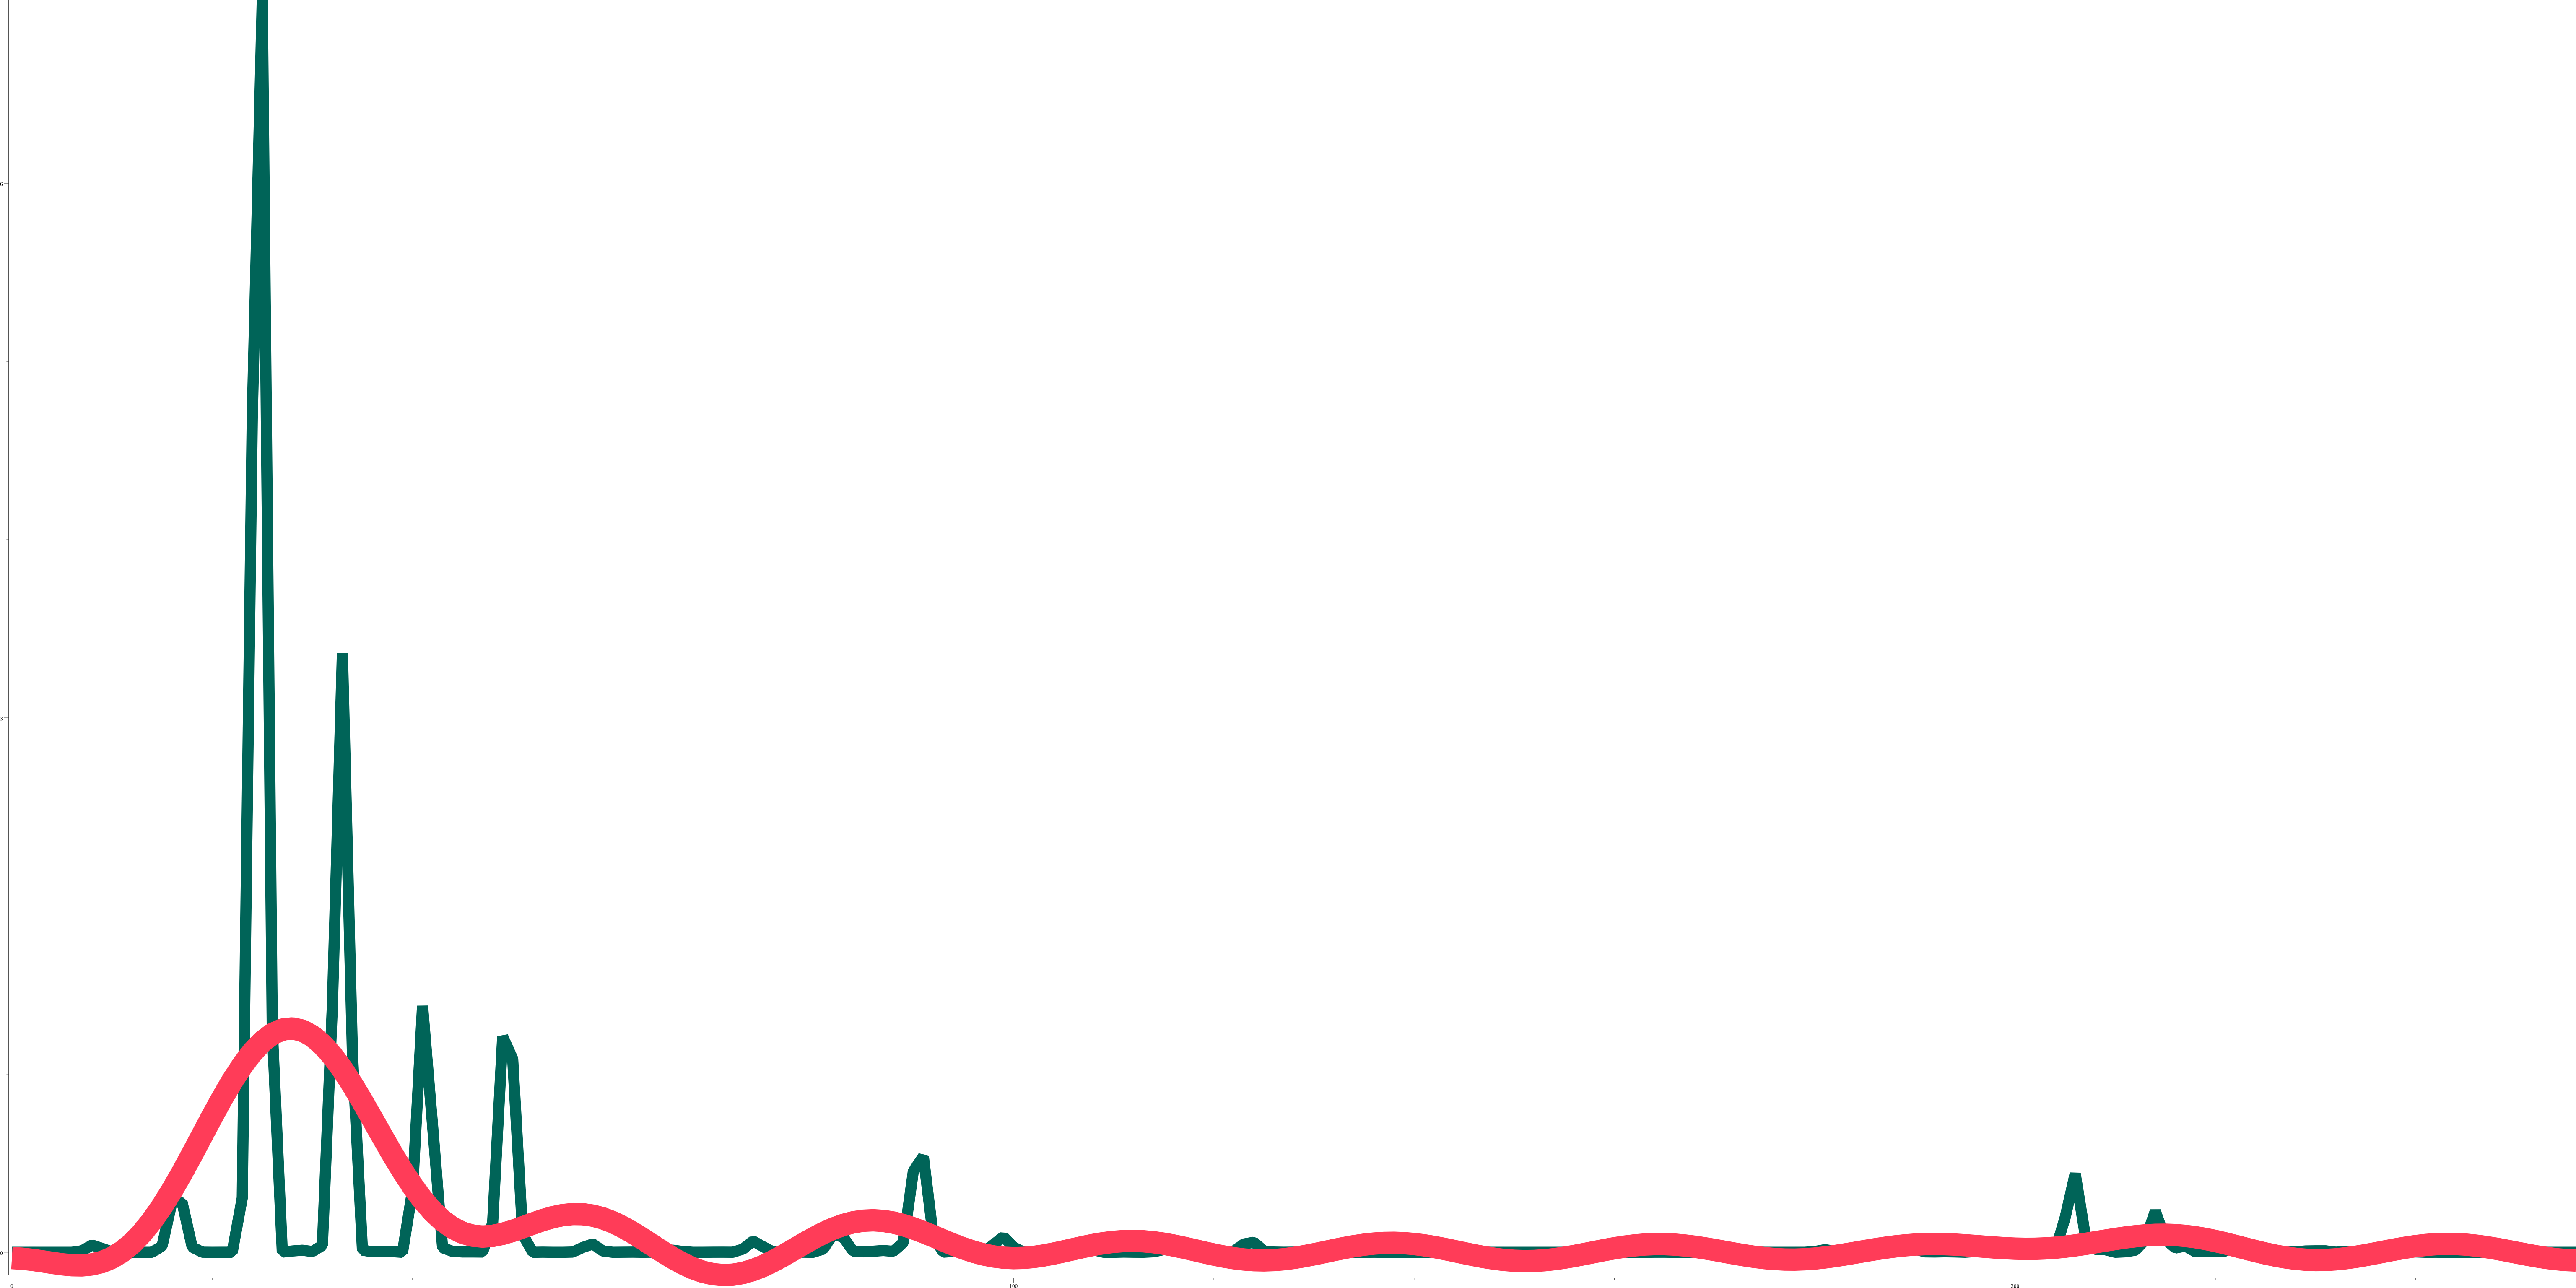
\includegraphics[width=\textwidth]{aaaa.png}
                    \end{column}
                    \pause
                    \hfill
                    \begin{column}{0.48\textwidth}
                         \includegraphics[width=\textwidth]{aaaa_log.png}
                    \end{column}
                \end{columns}
        }
        \only<5-11> {
            \item<5-11> Обратно Фурие преобразувание
            \item<6-11> $c_y[n] = c_g[n] + c_h[n]$
            \item<7-11> Кепстър
            \item<8-11> $c_g[n]$ ще са във високите честоти
            \item<9-11> $c_h[n]$ ще са в ниските
            \item<10-11> Използване на логаритимична (Мел) скала
            \item<11-11> Натрупване в критични области
        }
    \end{itemize}
\end{frame}

\begin{frame}
    \begin{itemize}
        \item Започваме от дискретен сигнал:
        
        \pause
        $s[n], n = 0, 1, \ldots, N$
        \item Разделяме сигнала $s[n]$ на фреймове:
        
        \pause
        $s_t[i] = s[tS + i]$,
        \pause
        \item Прилагаме прозоречна функция:
        
        \pause
        $x_t[n] = s_t[n]w_{hamming}[n]$, където
        \pause
        \item Намираме Фурие коефициентите:
        
        \pause
        $a_{k, t} = \cfrac{1}{L} \sum\limits_{n=0}^{L-1} x_t[n] e^{-\frac{2\pi i k n}{L}}$
        
        \pause
        \item Взимаме логаритъм от енергиите в критичните области: 
        
        \pause
        $c_{m, t} = \log\B{\sum\limits_{k = 0}^{L-1} |a_{k, t}|^2 H_{m}[k, f[m-1], f[m], f[m+1]]}, m = 0, 1, \ldots, M-1, M$-брой критични области.
        \pause
        
        \item Правим обратно преобразувание:
        \pause
        $mfcc_t[n] = \sum\limits_{m = 0}^{M-1} c_{m, t} cos(n\pi \cfrac{m+1/2}{M}), n = 0, 1, \ldots, M-1$
    \end{itemize}
\end{frame}

\begin{frame}[t]
    \begin{itemize}
        \item Гаусови смески
        \pause - всяко непрекъснато разпределение върху $\mathbb{R}^{n}$ може да се приближи произволно точно с линейна комбинация на достатъчно на брой гаусиани
        \pause
        \item За всяка емоция $e$ имаме по една смеска $(\hat{\pi}^e, \hat{\mu}^e, \hat{\Sigma}^e)$
        \pause
        \item При подаден характеристичен вектор $x$, вероятностната плътност на смеска е:
        \pause

        $p(x) = \sum\limits_{k=1}^{K} \pi_k^e \mathcal{N}(x; \mu_k^e, \Sigma_k^e)$
        \pause
        \item Правдоподобието на всички вектори X с етикет $e$ спрямо $(\hat{\pi}^e, \hat{\mu}^e, \hat{\Sigma}^e)$:
        \pause    
    
        $p(X|(\hat{\pi}^e, \hat{\mu}^e, \hat{\Sigma}^e)) = \prod\limits_{i=1}^{n} \sum\limits_{k=1}^{K} \pi_k^e \mathcal{N}(x_i; \mu_k^e, \Sigma_k^e)$.
        \pause
        \item За всяка емоция намираме Гаусовата смеска, която максимизира логаритъм от правдоподобието на съответните вектори
        \pause - ЕМ метод
        \pause
        \item За първоначално разбиване на векторите се ползва K-means++
    \end{itemize}
\end{frame}

    \begin{frame}[t]
        \begin{itemize}
            \item Emo-DB
            \pause - 800 записа от 10 актьори
        \end{itemize}
        \pause
        \begin{center}
            \resizebox{0.6\textwidth}{!}{\begin{tabular}{|l|r|r|} 
                \hline
                Емоция & Брой файлове & Обща дължина\\ 
                \hline
                Гняв & 127 & 5 мин. 35 сек.\\ 
                Щастие &  71 & 3 мин. 00 сек.\\ 
                Неутрално състояние &  79 & 3 мин. 06 сек.\\ 
                Тъга &  61 & 4 мин. 05 сек.\\ 
                \hline
            \end{tabular}}
        \end{center}
        \pause
        \begin{table}[h]
            \begin{center}
                \resizebox{\textwidth}{!}{\begin{tabular}{ |l|c|c|l| } 
                 \hline
                 Източник & Тип класификатор &  Тип характеристични вектори & Резултат \\ 
                 \hline
                 Текущ & GMM & MFCC & 82.20\% \\ 
                 2011 & SVM & LPCMFCC & 82.50\% \\ 
                 2006 &  Naïve Bayes classifier & MFCC & 82.76\% \\ 
                 2017 &  Random forest & MFCC & 79.02\% \\ 
                 \hline
                \end{tabular}}
                \caption*{Резултати върху emo-DB}
                \end{center}
        \end{table}
        \pause
        \begin{center}
            \resizebox{0.75\textwidth}{!}{\begin{tabular}{|l|r r r r|} 
                \hline
                & Гняв & Щастие & Неутрално & Тъга \\ 
                \hline
                Гняв &  \textbf{91.67\%} & 7.50\% & 0.00\% & 0.01\% \\ 
                Щастие & 37.14\% & \textbf{54.29\%} & 7.14\% & 1.43\% \\ 
                Неутрално & 0.00\% & 1.43\% & \textbf{82.86\%} & 15.71\% \\ 
                Тъга & 0.00\% & 0.00\% & 0.00\% & \textbf{100.00\%}\\ 
                \hline
                \hline
                Общо & & & & \textbf{82.20\%}\\
                \hline
            \end{tabular}}
        \end{center}
    \end{frame}

    \begin{frame}[t]
        \pause
        \begin{itemize}
            \item Тази сутрин-DB
        \end{itemize}
        \pause
        \begin{center}
            \resizebox{0.8\textwidth}{!}{\begin{tabular}{|l|r|r|} 
                \hline
                Емоция & Брой файлове & Обща дължина\\ 
                \hline
                Гняв & 51 & 4 мин. 15 сек.\\ 
                Щастие &  33 & 2 мин. 45 сек.\\ 
                Неутрално състояние &  18 & 1 мин. 30 сек.\\ 
                Тъга &  22 & 1 мин. 59 сек.\\ 
                \hline
            \end{tabular}}
        \end{center}
    \pause
    \begin{table}[h]
        \begin{center}
            \resizebox{0.8\textwidth}{!}{\begin{tabular}{|l|r r r r|} 
                \hline
                & Гняв & Щастие & Неутрално & Тъга\\ 
                \hline
                Гняв &  \textbf{72.00\%} & 4.00\% & 12.00\% & 12.00\%\\ 
                Щастие & 10.00\% & \textbf{73.33\%} & 0.00\% & 16.67\% \\ 
                Неутрално & 6.67\% & 6.67\% & \textbf{67.67\%} & 20.00\% \\ 
                Тъга & 0.00\% & 0.00\% & 0.00\% & \textbf{100.00\%}\\ 
                \hline
                \hline
                Общо & & & & \textbf{78.00\%}\\
                \hline
            \end{tabular}}
            \caption*{Матрица на грешките за база данни от ``Тази сутрин'' на ниво файл}
        \end{center}
        \end{table}
    \end{frame}

    \section{ЕЕГ}
    \begin{frame}[t]
        \center{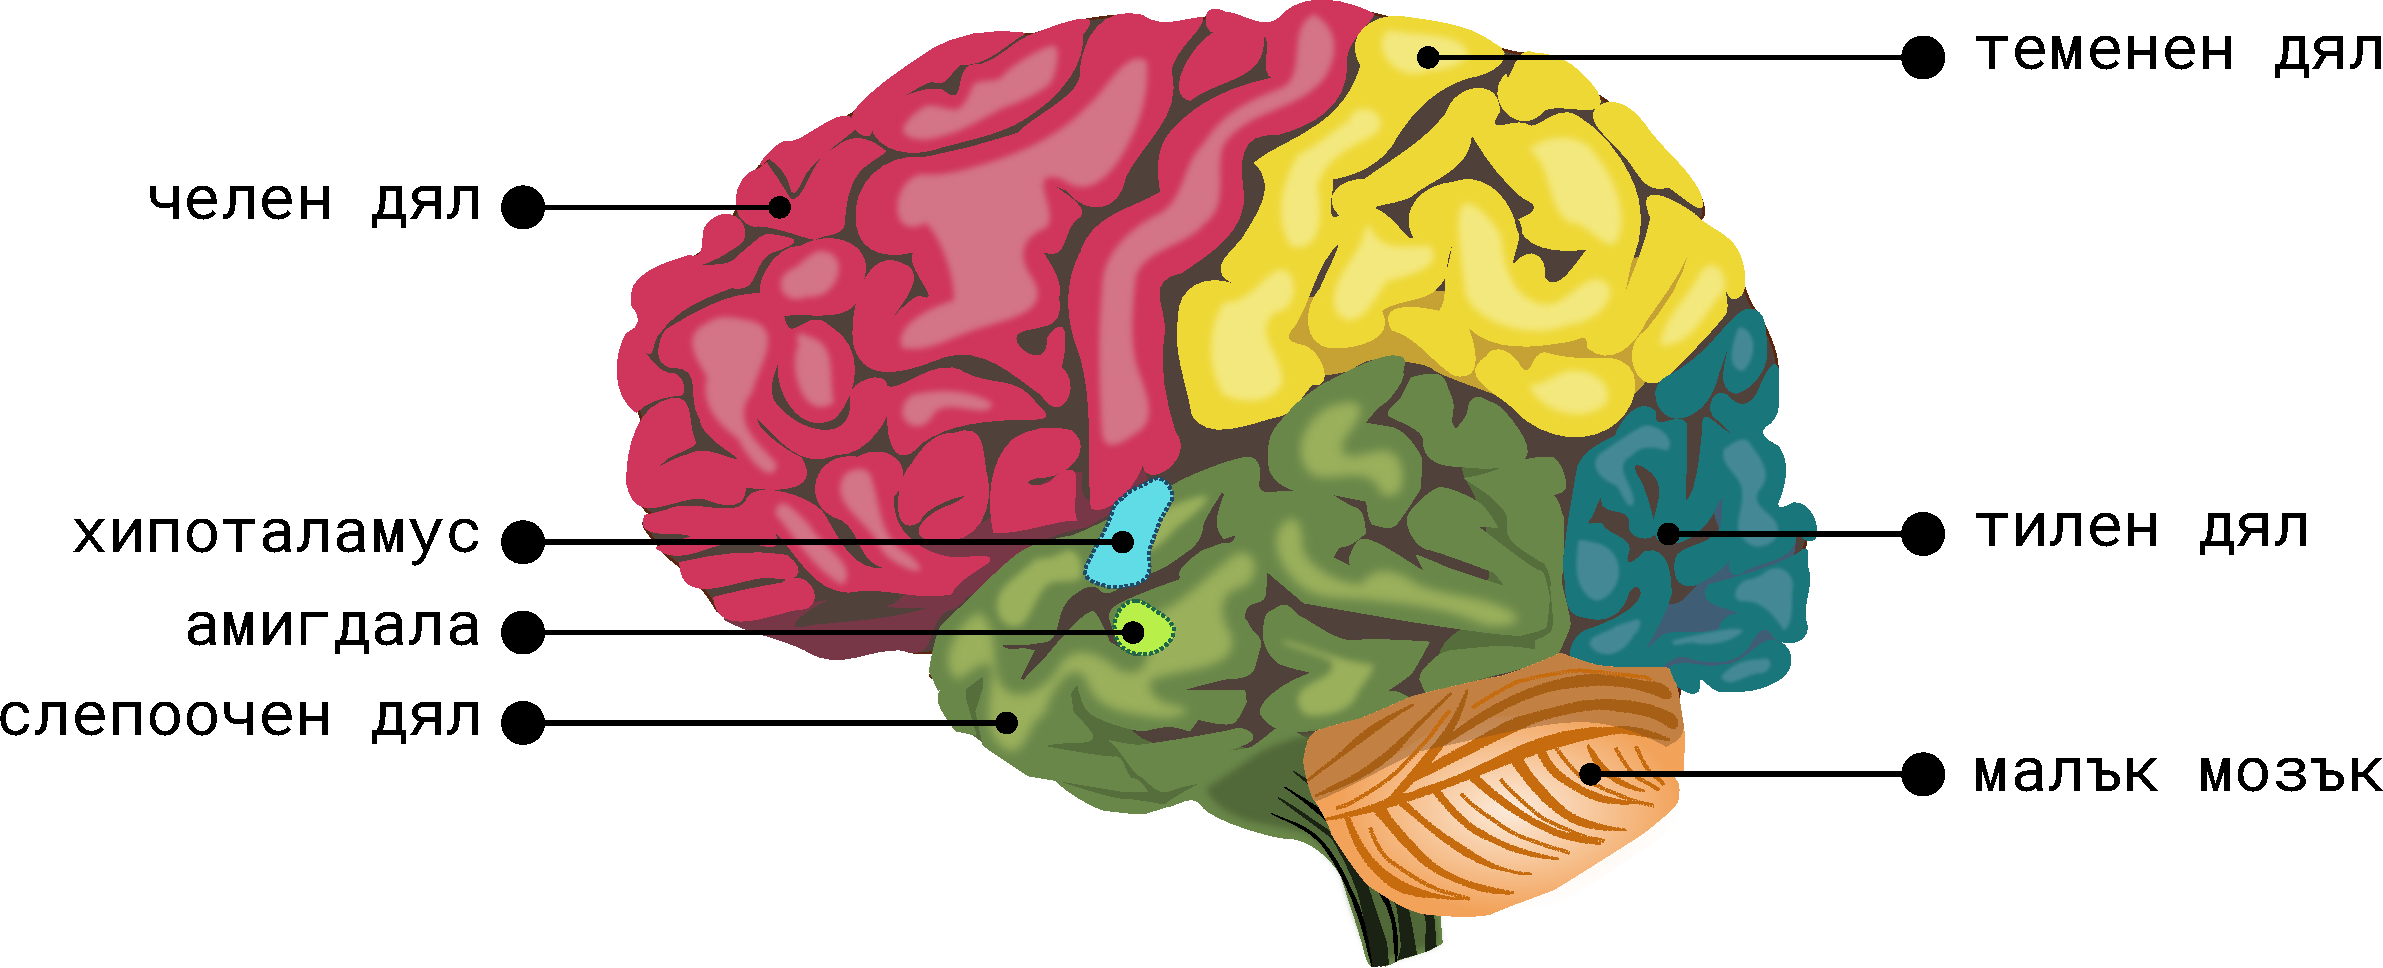
\includegraphics[width=0.75\paperwidth]{brain}}
        \only<2-4>{
            \begin{itemize}
                \item<2-4> Неврони - предават си електрически сигнали
                \item<3-4> Електроенцефалограф - измерва колебанията в напрежението на тези сигнали
                \item<4-4> Групиране на сигнала от ЕЕГ по полезни честотни ленти
            \end{itemize}
        }
        \only<5-9>{
            \begin{itemize}
                \item<5-9> $(1-4Hz)\ \delta$ вълни
                \item<6-9> $(4-8Hz)\ \theta$ вълни
                \item<7-9> $(8-12Hz)\ \alpha$ вълни
                \item<8-9> $(13-30Hz)\ \beta$ вълни
                \item<9-9> $(30-50Hz)\ \gamma$ вълни (ниски)
            \end{itemize}
        }
    \end{frame}
    
    \begin{frame}
        \only<1>{
            \center{
            \href{run:resources/gif/gif.mp4}{Видео}
            % \center{\animategraphics[loop,controls,width=0.9\linewidth]{2}{gif/all-}{0}{25}}
            }
        }
        \only<2>{
            \center{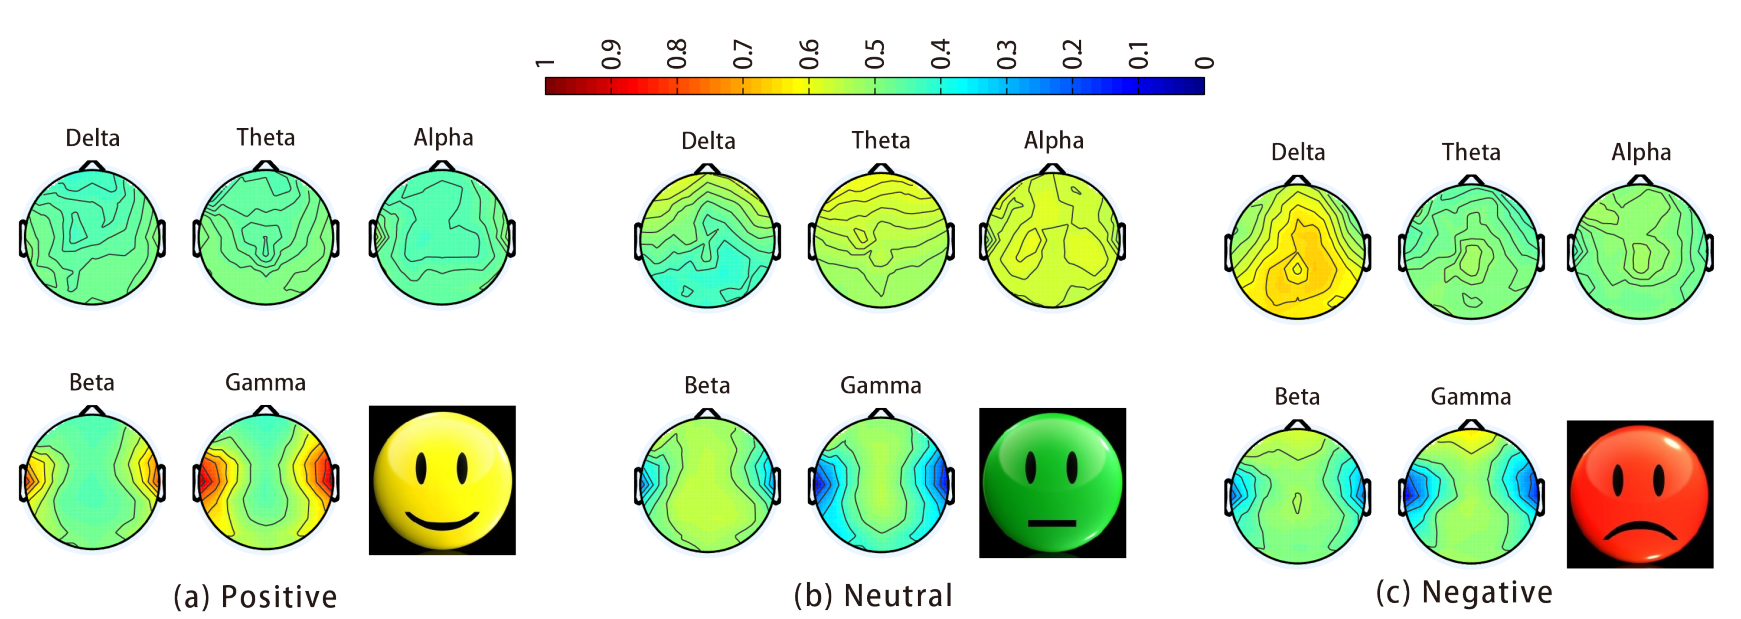
\includegraphics[width=0.8\paperwidth]{emotion_map.png}}
        }
    \end{frame}
    
    \begin{frame}[t]
        \begin{columns}
            \begin{column}{0.48\textwidth}
                \center{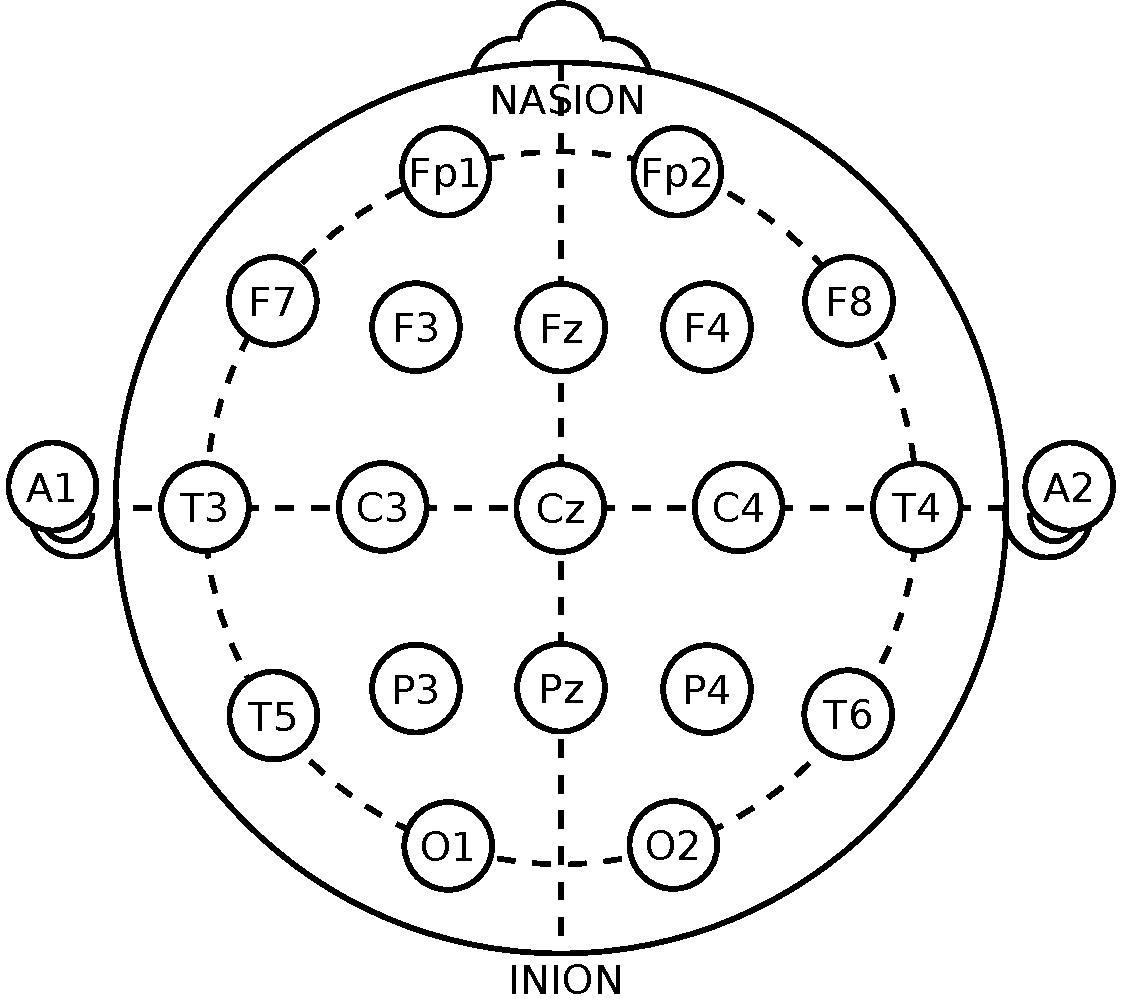
\includegraphics[width=0.8\textwidth]{10_20}}
            \end{column}
            \begin{column}{0.48\textwidth}
                \pause
                За характеристики ще ползваме енергията на  $\theta, \beta, \alpha, \gamma$ вълните.
                \pause
                Енцефалографът записва $500\times19$ мерни вектора в секунда.
            \end{column}
        \end{columns}
        \begin{itemize}
            \setlength\itemsep{\fill}
            \pause
            \item Прочитаме цялата информация за един електрод
            \pause
            \item Разделяме на фреймове с дължина $200ms$, взимайки ги през $150ms$, умножаваме по Хеминг прозорец и правим Фурие преобразувание
            \pause
            \item Сумираме енергиите на Фурие коефициентите в съответните 4 честотни банки, отговарящи на $\theta, \beta, \alpha, \gamma$ вълни
            \pause
            \item Получаваме F на брой $(19\times 4)$ мерни вектора
            \pause
            \item Класифицираме с Гаусови смески
        \end{itemize}
    \end{frame}

    \begin{frame}[t]{Опит едно}
        \center{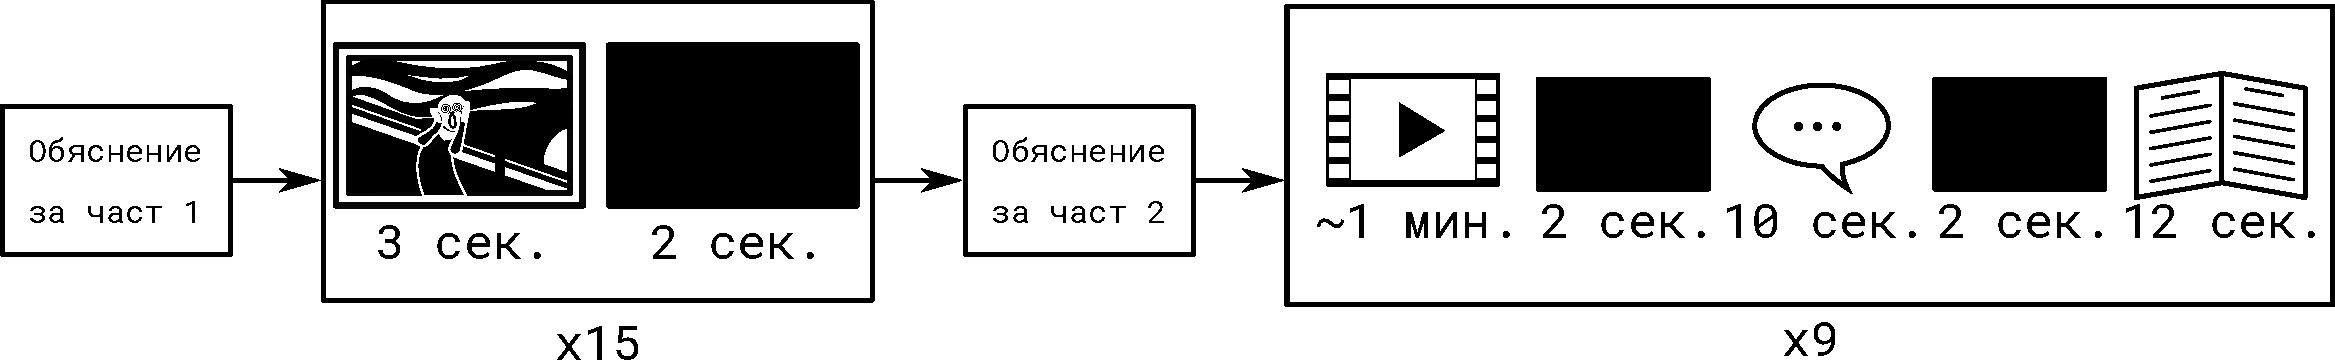
\includegraphics[width=\textwidth]{first_db}}
        \pause
        \begin{center}
        \begin{tabular}{|l|r|r|} 
            \hline
            Емоция & Брой файлове & Обща дължина\\ 
            \hline
            Гняв & 3 & 0 мин. 30 сек.\\ 
            Щастие & 3 & 0 мин. 30 сек.\\ 
            Неутрално състояние & 10 & 2 мин. 00 сек. \\ 
            Тъга & 4 & 0 мин. 40 сек. \\ 
            \hline
        \end{tabular}
        \pause
        \begin{table}[h]
            \begin{center}
            \begin{tabular}{|l|r r r r|} 
                \hline
                & Гняв & Щастие & Неутрално & Тъга \\ 
                \hline
                Гняв &  \textbf{33.33\%} & 0.00\% & 33.33\% & 33.33\% \\ 
                Щастие & 00.00\% & \textbf{100.00\%} & 0.00\% & 0.00\% \\ 
                Неутрално & 11.11\% & 0.00\% & \textbf{88.89\%} & 0.00\% \\ 
                Тъга & 0.00\% & 0.00\% & 100.00\% & \textbf{0.00\%}\\ 
                \hline
                \hline
                Общо & & & & \textbf{55.56\%}\\
                \hline
            \end{tabular}
            \caption*{Матрица на грешките от първия опит на ниво файл}
            \end{center}
        \end{table}
        \end{center}
    \end{frame}

    \begin{frame}[t]{Опит две}
            \begin{itemize}
                \pause
                \item Персонална постановка
                \pause
                \item Допълнителни стимули 
            \end{itemize}
            \pause
            \begin{center}
                \begin{tabular}{|l|r|r|} 
                    \hline
                    Емоция & Брой файлове & Обща дължина\\ 
                    \hline
                    Гняв & 18 & 6 мин. 53 сек.\\ 
                    Щастие & 0 & 0 мин. 00 сек. \\ 
                    Неутрално състояние & 31 & 8 мин. 12 сек. \\ 
                    Тъга & 45 & 15 мин. 13 сек. \\ 
                    \hline
                \end{tabular}
            \pause
            \begin{table}[h]
                \begin{center}
                    \begin{tabular}{|l|r r r r|} 
                        \hline
                        & Гняв & Щастие & Неутрално & Тъга \\ 
                        \hline
                        Гняв &  \textbf{100.00\%} & 0.00\% & 0.00\% & 0.00\% \\ 
                        Щастие & 00.00\% & \textbf{100.00\%} & 0.00\% & 0.00\% \\ 
                        Неутрално & 0.00\% & 0.00\% & \textbf{100.0\%} & 0.00\% \\ 
                        Тъга & 0.00\% & 0.00\% & 4.44\% & \textbf{95.56\%}\\ 
                        \hline
                        \hline
                        Общо & & & & \textbf{98.89\%}\\
                        \hline
                    \end{tabular}
                    \caption*{Матрица на грешките от втория опит на ниво файл}
                \end{center}
            \end{table}
            \end{center}
    \end{frame}

    \begin{frame}[c]
        \begin{center}
        \begin{table}[h]
            \begin{tabular}{|l|r r r r|} 
                \hline
                & Гняв & Щастие & Неутрално & Тъга \\ 
                \hline
                Гняв &  \textbf{80.33\%} & 5.00\% & 15.33\% & 0.00\% \\ 
                Щастие & 25.00\% & \textbf{75.00\%} & 0.00\% & 0.00\% \\ 
                Неутрално & 0.00\% & 2.50\% & \textbf{97.50\%} & 0.00\% \\ 
                Тъга & 0.00\% & 2.08\% & 10.42\% & \textbf{87.50\%}\\ 
                \hline
                \hline
                Общо & & & & \textbf{85.00\%}\\
                \hline
            \end{tabular}
            \caption*{Матрица на грешките при комбиниране на данните от първия и втория опит на ниво файл}
        \end{table}
        \end{center}
    \end{frame}

    \section{Реч и ЕЕГ}
    \begin{frame}[t]
        \begin{itemize}
            \item Идея едно
            \pause - конкатенираме характеристичните вектори от двата сигнала и тренираме нов класификатор
        \end{itemize}
        \pause
        \begin{table}[h]
            \begin{center}
                \resizebox{0.7\textwidth}{!}{\begin{tabular}{|l|r r r|}
                    \hline
                    Емоция    & Само реч         & Само ЕЕГ         & Конкатенация     \\
                    \hline
                    Гняв      & 85.00\%          & 80.00\%          & 86.50\%          \\
                    Щастие    & 75.00\%          & 75.00\%          & 57.50\%          \\
                    Неутрално & 7.50\%           & 97.50\%          & 91.75\%          \\
                    Тъга      & 85.42\%          & 87.50\%          & 81.04\%          \\
                    \hline
                    \hline
                    Общо      & \textbf{63.23\%} & \textbf{85.00\%} & \textbf{79.20\%} \\
                    \hline
                \end{tabular}}
                \caption*{Ниво файл}
            \end{center}
        \end{table}
        \pause
        \begin{table}[h]
            \begin{center}
                \resizebox{0.7\textwidth}{!}{\begin{tabular}{|l|r r r|}
                    \hline
                    Емоция    & Само реч         & Само ЕЕГ         & Конкатенация     \\
                    \hline
                    Гняв      & 41.53\%          & 53.05\%          & 68.07\%          \\
                    Щастие    & 37.35\%          & 44.44\%          & 34.55\%          \\
                    Неутрално & 32.91\%           & 66.72\%          & 68.58\%          \\
                    Тъга      & 39.66\%          & 70.38\%          & 68.04\%          \\
                    \hline
                    \hline
                    Общо      & \textbf{37.86\%} & \textbf{58.65\%} & \textbf{59.81\%} \\
                    \hline
                \end{tabular}}
                \caption*{Ниво вектор}
            \end{center}
        \end{table}
    \end{frame}

    \begin{frame}[t]
        \begin{itemize}
            \setlength\itemsep{\fill}
            \item Идея две
            \pause - максимизиране на правдоподобието/ентропията
            \pause
            \item Ако имаме входни данни $\mathcal{D} = (x_1, y_1),\ldots,(x_n, y_n)$, където $x_i \in \mathbb{R}^n$ са характеристични вектори с етикети $y_i \in Y=\{1,\ldots, K\}$
            \pause
            \item Ако означим двата си класификатора съответно с $h_1, h_2: X\times Y \rightarrow [0, 1]$
            \pause
            \item Търсим разпределение над $X\times Y$, което:
            
            \pause - се държи като емпиричното разпределение върху дадените данни
            
            \pause - очакването на $h_i$, спрямо разпределението, съвпада с очакването на емпиричното
            \pause - $E(p, h) = \sum\limits_{(x, y) \in X\times Y} p(x, y)h(x, y)$

            \pause - не внася допълнителни предположения извън тренировъчното множество
            \pause
            \item Принцип за максимизиране на ентропията
            \pause - като правим заключения на базата на частична информация, трябва да използваме това разпределение, което има максимална ентропия, спрямо известните величини.
        \end{itemize}
    \end{frame}


    \begin{frame}[t]
        \begin{itemize}
            \setlength\itemsep{\fill}
            \item Може да се покаже, че това разпределение максимизира логаритъм от условното правдоподобие
            \pause $\log\B{\widehat{L}_{\mathcal{D}}(Y|X)} = \sum\limits_{(x, y) \in X\times Y} \#(x, y) p(y|x)$
            \pause
            \item Търсеното разпределение има вида:
            \pause
            \[\hat{p}(y|x) = \cfrac{exp\B{\lambda_1 h_1(x, y) + \lambda_2 h_2(x, y)}}{\sum\limits_{y' \in Y} exp\B{\lambda_1 h_1(x, y') + \lambda_2 h_2(x, y')} }\]
            \pause
            \item Намираме $\lambda_1, \lambda_2$ с градиентен метод, максимизирайки логаритъм от правдоподобието
            \pause
            \item Получаваме следния класификатор:
            \pause \[H(x) = argmax_{y\in Y} \B{\lambda_1 h_1(x, y) + \lambda_2 h_2(x, y)}\]
        \end{itemize}
    \end{frame}

    \begin{frame}[t]{Съчетаване на двата сигнала}
        \begin{table}[h]
        \pause
        \begin{center}
            \begin{tabular}{|l|r r r|}
                \hline
                Емоция    & Само реч         & Само ЕЕГ         & Комбинация     \\
                \hline
                Гняв      & 85.00\%          & 80.00\%          & 80.00\%          \\
                Щастие    & 75.00\%          & 75.00\%          & 75.00\%          \\
                Неутрално & 7.50\%           & 97.50\%          & 97.50\%          \\
                Тъга      & 85.42\%          & 87.50\%          & 87.50\%          \\
                \hline
                \hline
                Общо      & \textbf{63.23\%} & \textbf{85.00\%} & \textbf{85.00\%} \\
                \hline
            \end{tabular}
            \caption*{Ниво файл}
        \end{center}
        \end{table}
        \pause
        \begin{table}[h]
            \begin{center}
                \begin{tabular}{|l|r r r|}
                    \hline
                    Емоция    & Само реч         & Само ЕЕГ         & Комбинация     \\
                    \hline
                    Гняв      & 41.53\%          & 53.05\%          & 53.30\%          \\
                    Щастие    & 37.35\%          & 44.44\%          & 44.09\%          \\
                    Неутрално & 32.91\%           & 66.72\%          & 66.46\%          \\
                    Тъга      & 39.66\%          & 70.38\%          & 71.07\%          \\
                    \hline
                    \hline
                    Общо      & \textbf{37.86\%} & \textbf{58.65\%} & \textbf{58.73\%} \\
                    \hline
                \end{tabular}
                \caption*{Ниво вектор}
            \end{center}
        \end{table}
    \end{frame}
    \begin{frame}[t]{Заключение}
        \pause
    \end{frame}
\end{document}